\usetikzlibrary{patterns}
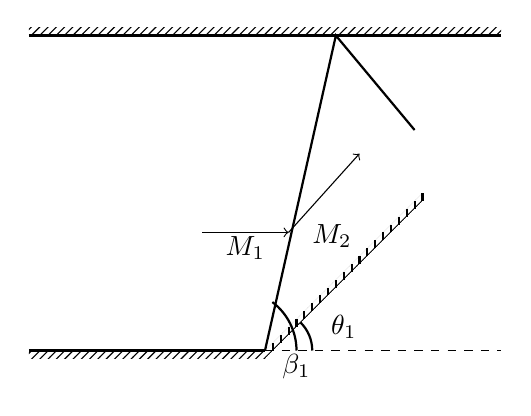
\begin{tikzpicture}
    \fill[pattern=north east lines] (-3,3.1) rectangle (3,3); 
    \fill[pattern=north east lines] (-3,-1) rectangle (0,-1.1); 
\draw[thick] (0.1,-1) -- (0.1,-0.9);
\draw[thick] (0.2,-0.9) -- (0.2,-0.8);
\draw[thick] (0.3,-0.8) -- (0.3,-0.7);
\draw[thick] (0.4,-0.7) -- (0.4,-0.6);
\draw[thick] (0.5,-0.6) -- (0.5,-0.5);
\draw[thick] (0.6,-0.5) -- (0.6,-0.4);
\draw[thick] (0.7,-0.4) -- (0.7,-0.3);
\draw[thick] (0.8,-0.3) -- (0.8,-0.2);
\draw[thick] (0.9,-0.2) -- (0.9,-0.1);
\draw[thick] (1,-0.1) -- (1,0);
\draw[thick] (1.1,0) -- (1.1,0.1);
\draw[thick] (1.2,0.1) -- (1.2,0.2);
\draw[thick] (1.3,0.2) -- (1.3,0.3);
\draw[thick] (1.4,0.3) -- (1.4,0.4);
\draw[thick] (1.5,0.4) -- (1.5,0.5);
\draw[thick] (1.6,0.5) -- (1.6,0.6);
\draw[thick] (1.7,0.6) -- (1.7,0.7);
\draw[thick] (1.8,0.7) -- (1.8,0.8);
\draw[thick] (1.9,0.8) -- (1.9,0.9);
\draw[thick] (2,0.9) -- (2,1);

    \draw[dashed] (0,-1) -- (3,-1);
    \draw[thick] (-3,-1) -- (0,-1);
    \draw[thick] (-3,3) -- (3,3);

    \fill[pattern=north east lines] (0,-1) -- (2,1) -- (2,0.9) -- (0,-1.1) -- cycle;

    \draw [thick](0,-1) -- (0.9,3) -- (1.9,1.8);
    \draw[->] (-0.8,0.5) -- (0.3,0.5);
    \node at (-0.25,0.3) {$M_1$};
    \draw[->] (0.3,0.5) -- (1.2,1.5);
    \node at (0.85,0.455) {$M_2$};

    \draw[thick] (0.4,-1) arc[start angle=0, end angle=53, radius=0.77];
    \node at (0.4,-1.2) {$\beta_1$};
    \draw[thick] (0.6,-1) arc[start angle=0, end angle=45, radius=0.5];
    \node at (1,-0.7) {$\theta_1$};
\end{tikzpicture}
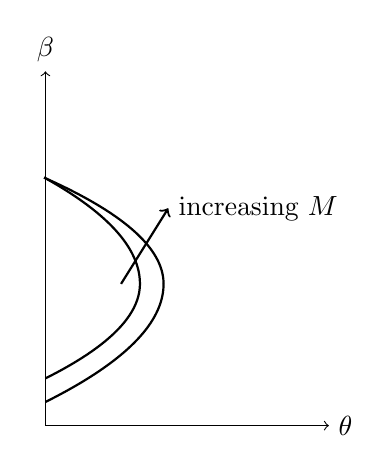
\begin{tikzpicture}[scale=1.2]
    \draw[->] (0,0) -- (0,3.75) node[above] {$\beta$};
    \draw[->] (0,0) -- (3,0) node[right] {$\theta$};
        \draw[thick, domain=0:4.5, smooth, variable=\y] plot ({1.25 - 0.0625*\y^2}, {0.25*\y+1.5});
    \draw[thick, domain=0:4.5, smooth, variable=\y] plot ({1 - 0.05*\y^2}, {0.25*\y+1.5});
     \draw[thick, domain=-4:0, smooth, variable=\y] plot (-{1.25 + 0.0625*\y^2}+2.25, {0.25*\y+1.5});
    \draw[thick, domain=-5:0, smooth, variable=\y] plot (-{1 + 0.05*\y^2}+2.25, {0.25*\y+1.5});
    \draw[->, thick] (0.8,1.5) -- (1.3,2.3) node[right] {increasing $M$};
\end{tikzpicture}

